\documentclass[reprint,amsmath,amssymb]{revtex4-1}
\usepackage{graphicx,natbib,overpic,xcolor}
\bibliographystyle{unsrtnat}
\begin{document}

\title{Line formation and cavity growth in LES data} % Cold pool collisions

\author{Silas Boye Nissen}
\affiliation{Niels Bohr Institute \\ University of Copenhagen \\ Blegdamsvej 17, 2100
Copenhagen \\ Denmark \\}

\author{Jan O.~Haerter}
\email{haerter@nbi.ku.dk}
\affiliation{Niels Bohr Institute \\ University of Copenhagen \\ Blegdamsvej 17, 2100
Copenhagen \\ Denmark \\}

\date{\today}

\begin{abstract} % on the order of 150 words
% KEY POINTS
% (1) initial pattern non-random
% (2) ormation of lines
% (3) run-away growth of large cavities
Typically, convective self-aggregation proceeds over 10---100 days in radiative convective equilibrium (RCE) simulations \cite{wing2017convective}.
In RCE, the initial pattern of convective cells is often considered to be un-organized, or random \cite{hohenegger2016coupled}. 
Eventually, sub-regions gradually form, where convection is not present, breaking the initial symmetry. 
%The standard theory for convective self-aggregation invokes radiation feedback, which cause cloudless subregions to experience subsidence and near surface divergence, whereas already cloudy regions are reinforced. 
Here, we show that the pattern of cells is already non-random few hours after the initial onset of convection: 
cloud patterns organize into line structures, shown here by analysis of high-resolution large-eddy simulations. 
The formation of such lines is hard to explain without the specific interaction between cold pool gust fronts, namely one where two cold pools collide to form a new cloud in between \cite{tompkins2001organizationCold,boing2016object,haerter2018reconciling,de2017cold}. 
By tracking cold pools, we determine their maximal radii  $r_{max}\sim 20\;km$, and show that cloud free regions exceeding such radii always grow indefinitely, while smaller ones often decay. 
Our theory suggests a mechanistic theory, where cloud free regions in RCE are likely to form, when cold pools have small $r_{max}$ and cannot replicate, whereas large $r_{max}$ hampers such cavities. 
Our findings imply, that the dynamics of self-aggregation is crucially controlled by cold pool interaction and known feedbacks may only be required in stabilizing the final, fully-aggregated state. 
%Here, we bring forward a new mechanism, by which cold pool properties alone can determine, whether a tropical sea surface will be covered by aggregated or unorganized convection. Our conceptual model closely agrees with large eddy simulations and predicts that line structures of organized cloud patterns form as a simple conference of the characteristic interactions between cold pools. Over time, cavities of cloudless regions self-organize, ultimately resulting in the canonical segregation typical of radiative convective equilibrium simulations. Our results imply that the role of cold pools on self-aggregation may currently be underestimated.
\end{abstract}

\maketitle

\section{Introduction}
When rain evaporation is strong, so is cooling and sub-cloud density increase \cite{simpson1980downdrafts,engerer2008surface}, forcing the resulting cold pools to spread quickly and cover larger distances \cite{romps2016sizes,torri2015mechanisms,zuidema2017survey}.
Such strong cold pool activity has repeatedly been suggested to hamper convective self-aggregation in RCE numerical experiments \cite{jeevanjee2013convective,muller2015favors,holloway2016sensitivity,hohenegger2016coupled}.
%Convective self-aggregation is a form of symmetry breaking in long, convection permitting, simulations of the convective atmosphere under constant sea surface conditions and constant insolation, under the absence of external wind shear \cite{held1993radiative,tompkins1998radiative,bretherton2005energy,hohenegger2016coupled,wing2017convective}.
%In such simulations, over typical temporal scales of days to weeks, the energy fluxes entering and leaving the system approach an approximate equilibrium state.
In these simulations, the atmosphere gradually organizes from an initial, apparently random, pattern of convective updrafts into an inhomogeneous pattern with one or few strongly convecting patches, but an otherwise nearly precipitation free domain \cite{held1993radiative,tompkins1998radiative,bretherton2005energy,hohenegger2016coupled,wing2017convective}. 
When rain evaporation is removed, self-aggregation was found to be favored.
%As they do so, the pattern formed by convective precipitation cells gradually organizes from an initial, apparently random, pattern to a segregated one, where the domain is sub-divided into a strongly precipitating patch and an otherwise nearly rain-free area. {\color{red} Silas: I think the abstract and this first introduction paragraph need to be even more sharp and precise. Let's discuss this...}

Physical processes discussed as contributing to self-aggregation are positive feedback between latent and sensible heat fluxes, radiation, and clouds, as well as their influence on the atmospheric circulation. ´
The early stage of self-aggregation is characterized by the appearance of small dry regions, within which rain is suppressed \citep{holloway2017observing}.
Along with this suppression, further drying was reported to occur through radiative cooling and the resulting subsidence, as well as changes in surface fluxes.
In the later stage, dry patches expand and merge, eventually leaving only one contiguous moist region.
A remarkable aspect of self-aggregation is hysteresis, by which it refuses to disaggregate, once formed, even when initially-required feedback are removed \cite{khairoutdinov2010aggregation,muller2012detailed,muller2015favors}.

%One particular dynamical aspect to convection are so-called cold pools, which are formed under precipitating convective clouds, when the clouds' rain evaporates before reaching the surface \cite{simpson1980downdrafts,engerer2008surface}.
Cold pools are capable of mediating organization, as they effectively handing on "information" between one precipitating cloud and its surroundings.
Physically, cold pools spread as density currents along the surface, carry kinetic energy and can modify the thermodynamic structure of the environment near their edges \cite{tompkins2001organizationCold,langhans2015origin,de2017cold}.
Cold pools can then act to pattern the convectively unstable atmosphere, as the loci where new convective cells emerge, is not independent of the loci at which previous cell dissipate.
In particular, new cells were suggested to be spawned by the cold pool gust front alone, or by collisions between mobile gust fronts \cite{de2017cold,glassmeier2017network,cafaro2018characteristics}, and several conceptual studies, formulating cold pools as cellular automata, have resulted from the notion of cold pool interactions \cite{grandpeix2010density,boing2016object,haerter2018reconciling}.
% re-upload the ARXIV or cite the other GRL !!

%Time periods required for the emergence of a fully aggregation state vary by an order of magnitude \cite{wing2017convective}, and can be shorter, when cold pools are suppressed \cite{jeevanjee2013convective,holloway2016sensitivity}.
%Strong cold pools hence appear to hinder self-aggregation, the domain will continue to experience apparently unorganized convection, without the run-away broken-symmetry state.
%If interactions between cold pools are relevant in stimulating new convective cells, in how far can a suppression of cold pools then favor self-aggregation?
%This is the question addressed in the current work.

We analyse large eddy simulations by which cold pool gust fronts, their spreading and interaction can be resolved sufficiently (Fig.~\ref{fig:cavities}a, {\it Details:} Methods).
By constructing a cold pool tracking method, where particles are placed at the edge of active precipitation cells and advected with the horizontal flow surrounding these precipitation cells, we are able to track the evolution of these cold pools.
Indeed, cold pools predictably form shortly after rain falls through the boundary layer, and initially spread horizontally at speeds of approximately 3 $m\;s^{-1}$.
However, due to frictional forces and mixing, cold pools do not grow indefinitely -- in our simulations, they typically do not exceed radii of $r_{max}= 20\;km$, a value commensurate with previous simulations \cite{romps2016sizes} and observations \cite{black1978mesoscale,zuidema2012trade,feng2015mechanisms}.

When examining our simulations, new precipitation cells often emerge in close proximity to the interfaces between the gust fronts from two distinct cold pools.
These gust fronts have usually become immobile by the time a new precipitation event emerges.
The time delay can be as large as 3--5 hours {\color{red} [make this more precise, if possible]}.
Despite this delay, the location of newly emerging cells is systematically positioned near the collision lines formed by previous cold pool gust fronts, a non-random organizational pattern should hence be expected.

\section{Results}
We first characterize the patterning observed in the spatial distribution of precipitation cells in a 30-day simulation of convective self-aggregation.
We discuss the formation and dynamics of dry patches and the appearance of marked, non-random, line-segments, which connect precipitation cell centers and are often nearly perfectly straight.
To explain both features, we then bring forward a simple model, based on the interaction of expanding circles, which captures the interaction between cold pool gust fronts and their spawning of subsequent precipitation events.

\subsection{Cavities need a critical size to either grow or die}
When tracking the cavities present in the domain at any time step, an initial population of relatively small cavities is already present two days after the onset of precipitation.
%{\color{red} Silas: Would it be good to show snapshots at 6 different time points of the LES data in the supplement (or a movie)?}
When following the growth of these cavities, some reach larger sizes and eventually contain points that exceed a critical distance $d_0>r_{max}$ (Figs~\ref{fig:cavities} and ~\ref{fig:cavities_supp}).
We identify a characteristic value of $r_{max} \approx 22.5$ $km$, for which it is found that essentially all cavities containing points with $d_0>r_{max}$ grow indefinitely, that is, their areas grow without bound.
Cavities for which all points lie below this threshold, may decay in area.
Unbounded growth of some cavities requires that merging events take place, whereby multiple cavities connect to form even larger ones.

\begin{figure*}
\centering
%\begin{overpic}
%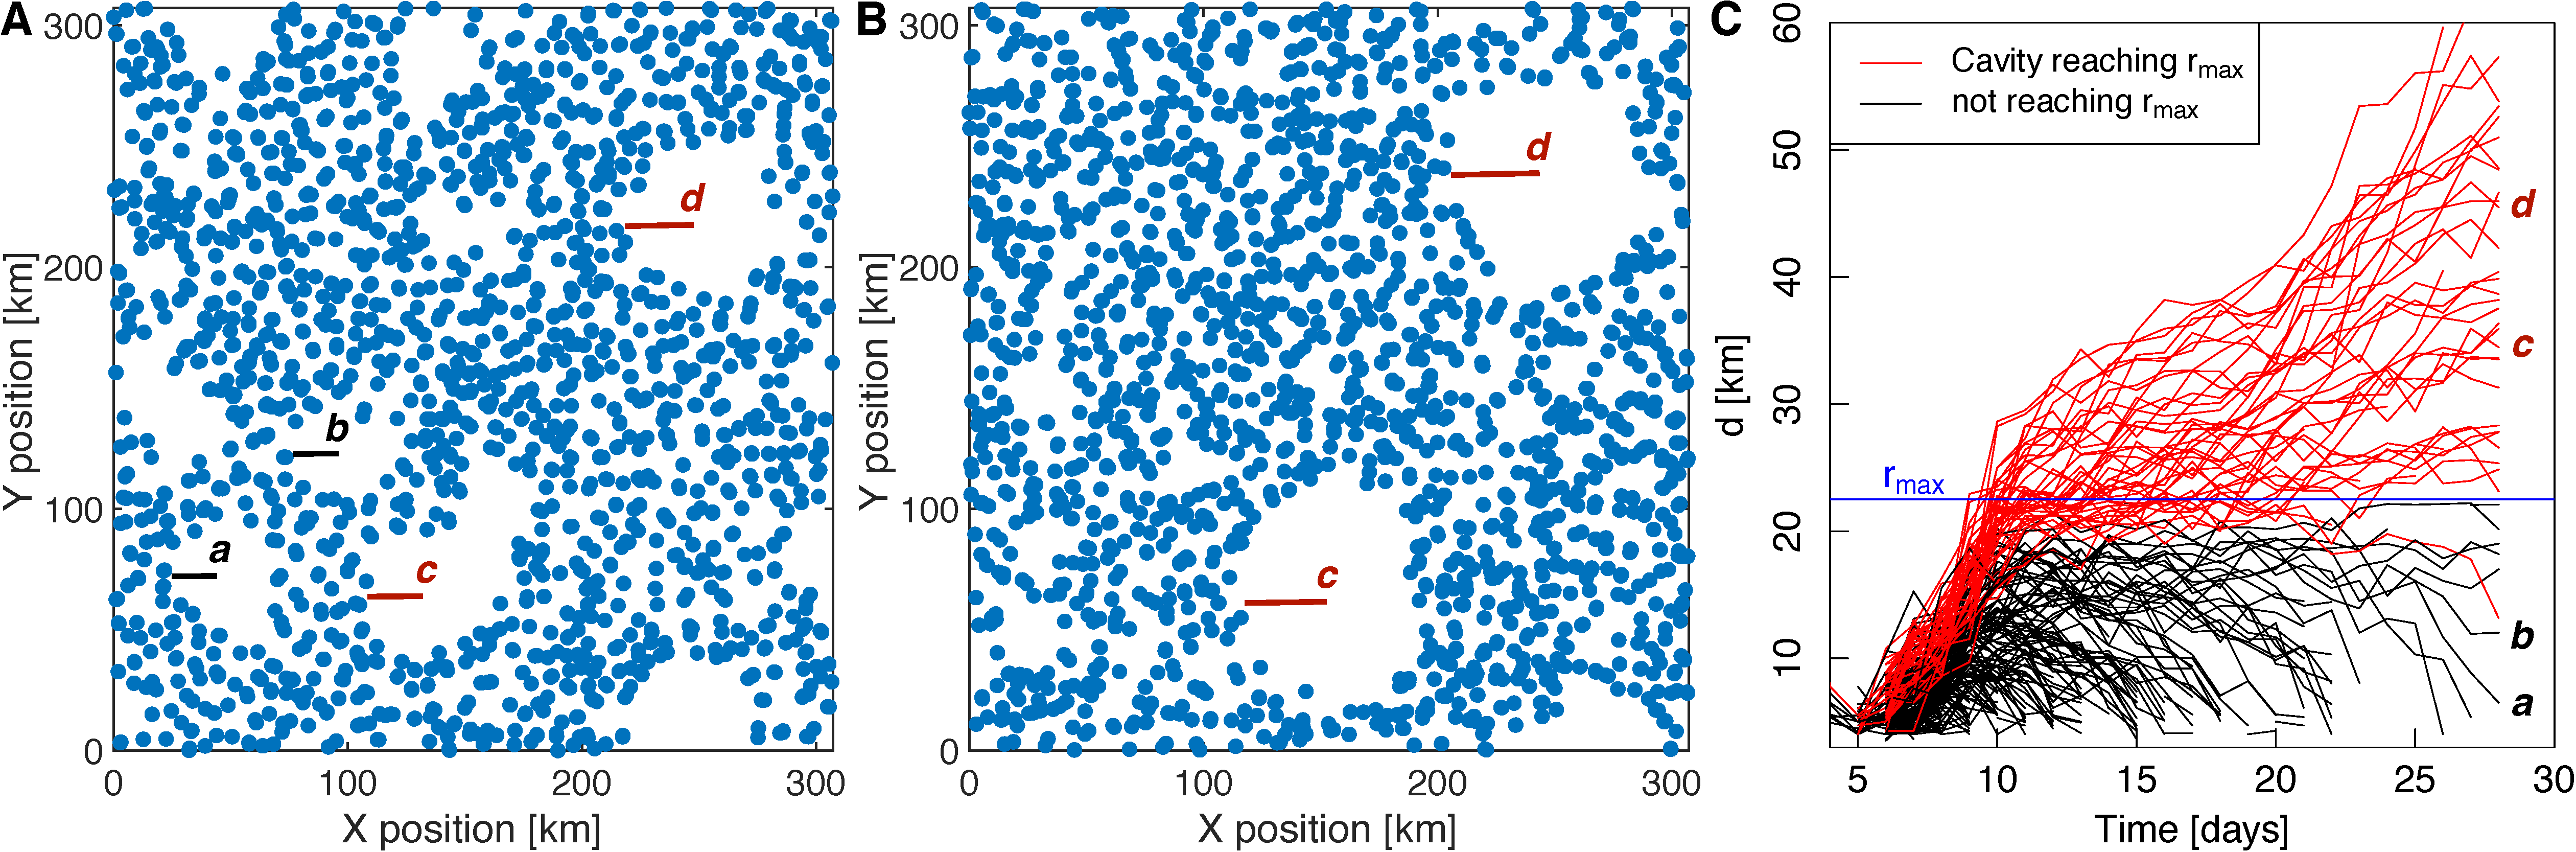
\includegraphics[height=0.33\linewidth]{cavities}
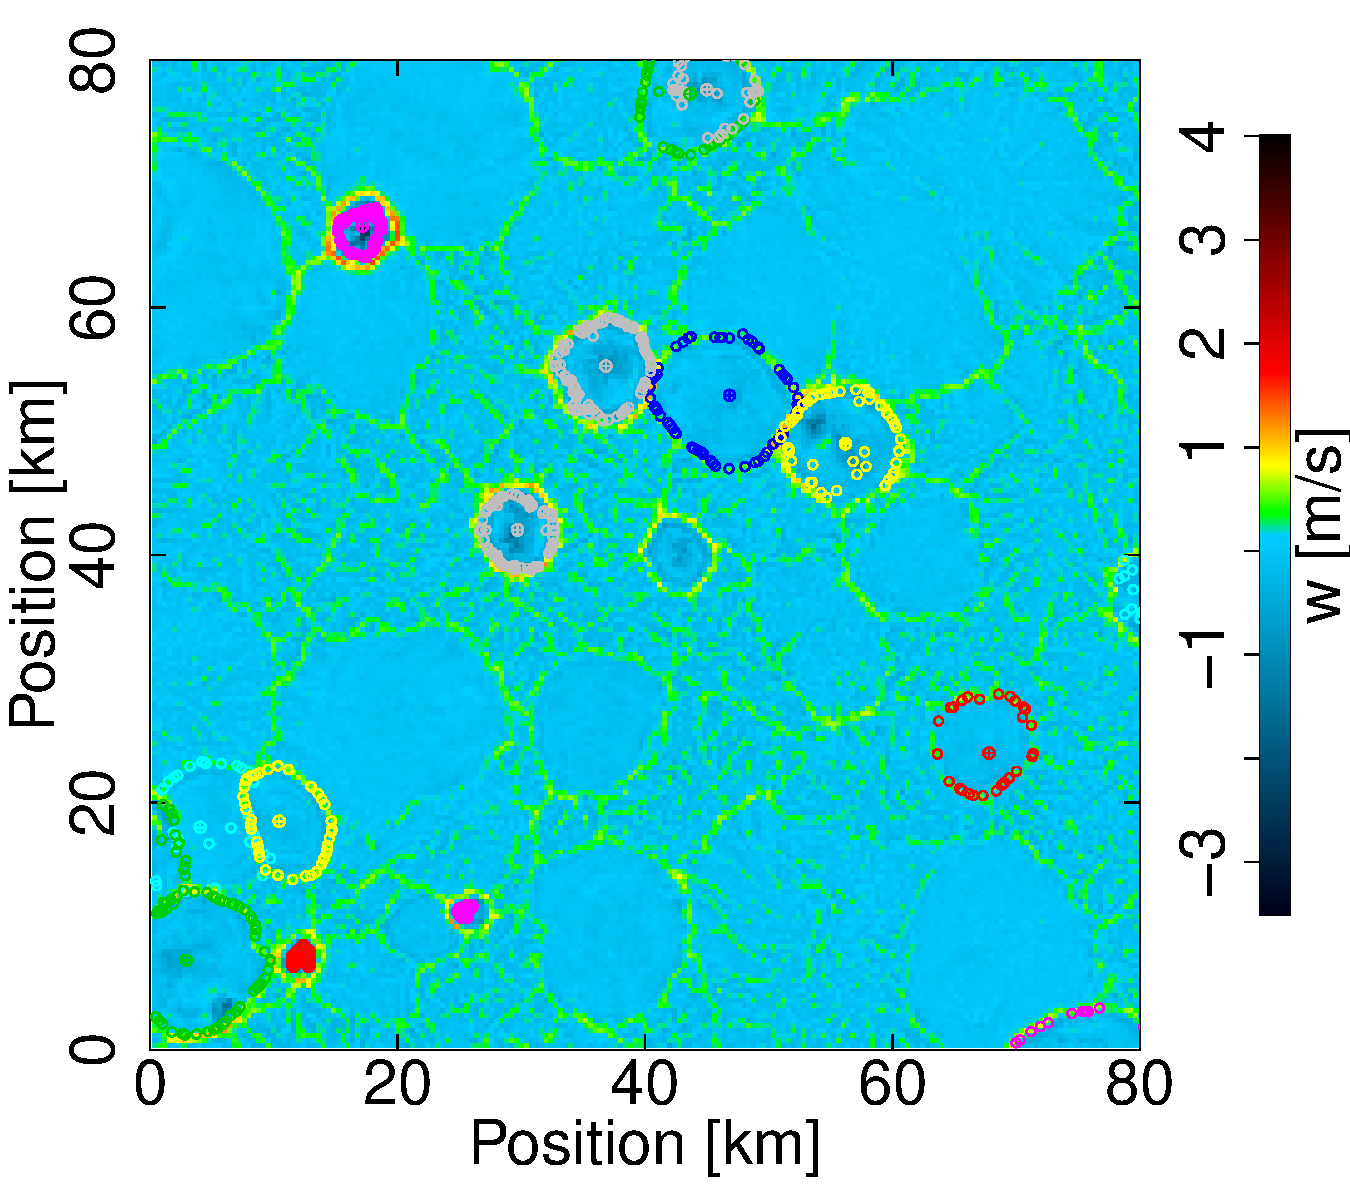
\includegraphics[height=0.32\linewidth]{spaceplot_t=15.pdf}
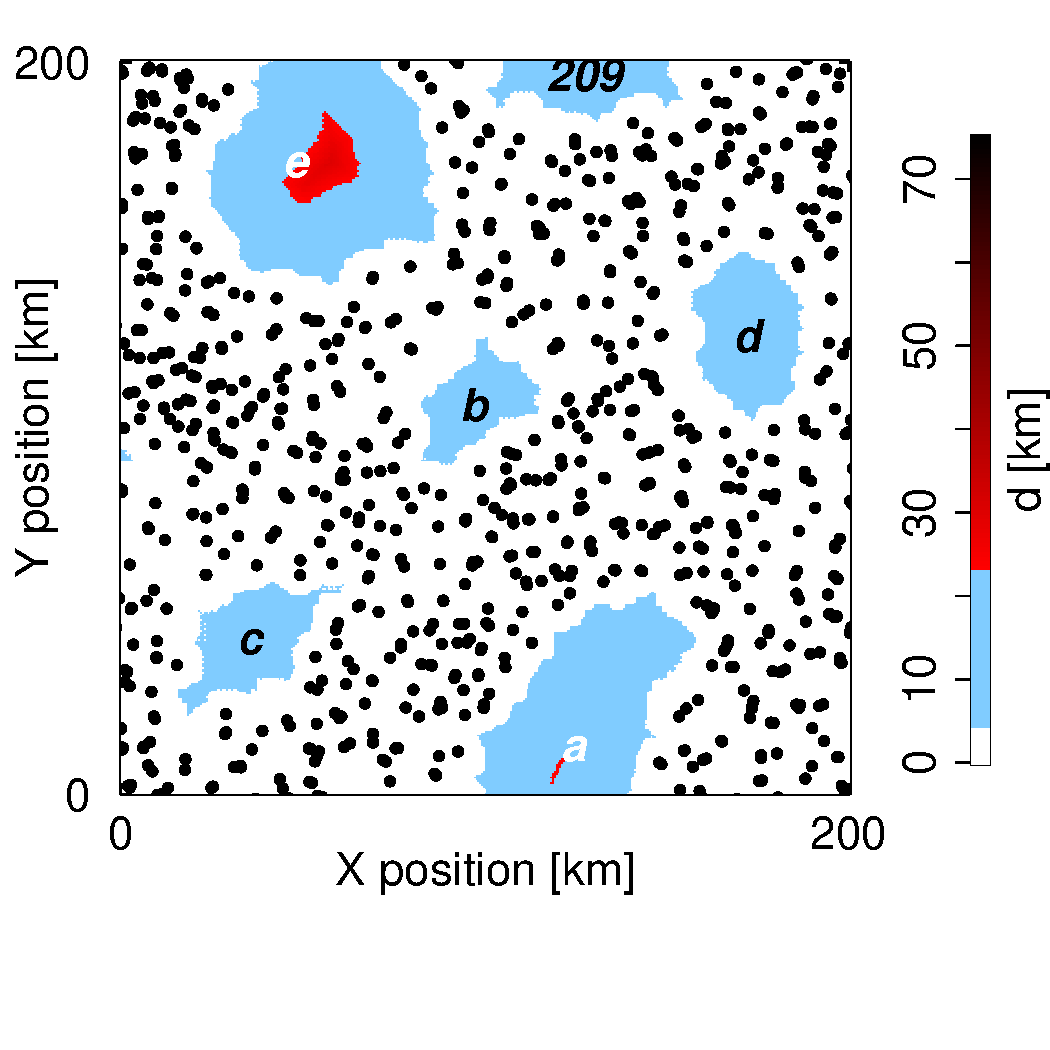
\includegraphics[trim={0 0 2.8cm 0}, clip, height=0.38\linewidth]{distance_13.pdf}
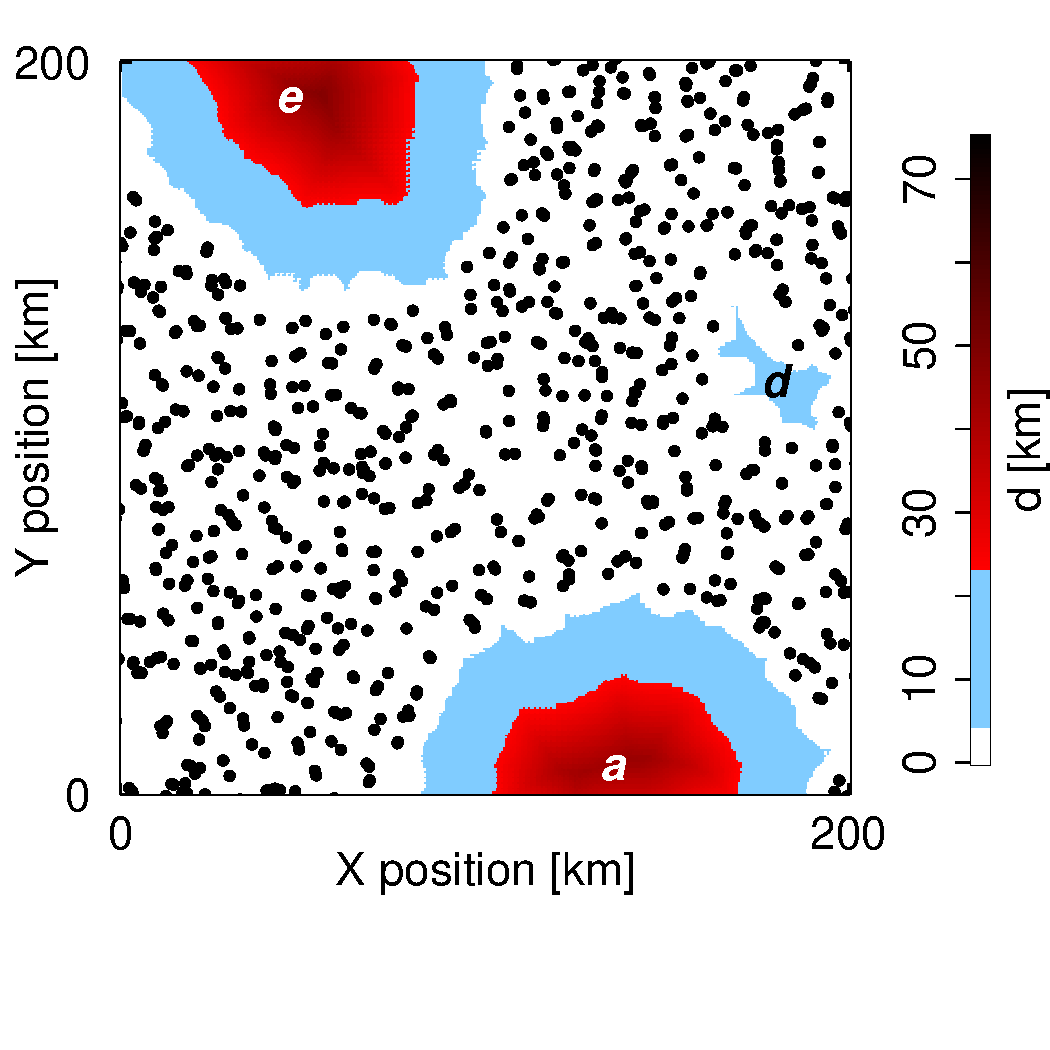
\includegraphics[trim={1.5cm 0 2.8cm 0}, clip, height=0.38\linewidth]{distance_25.pdf}\\
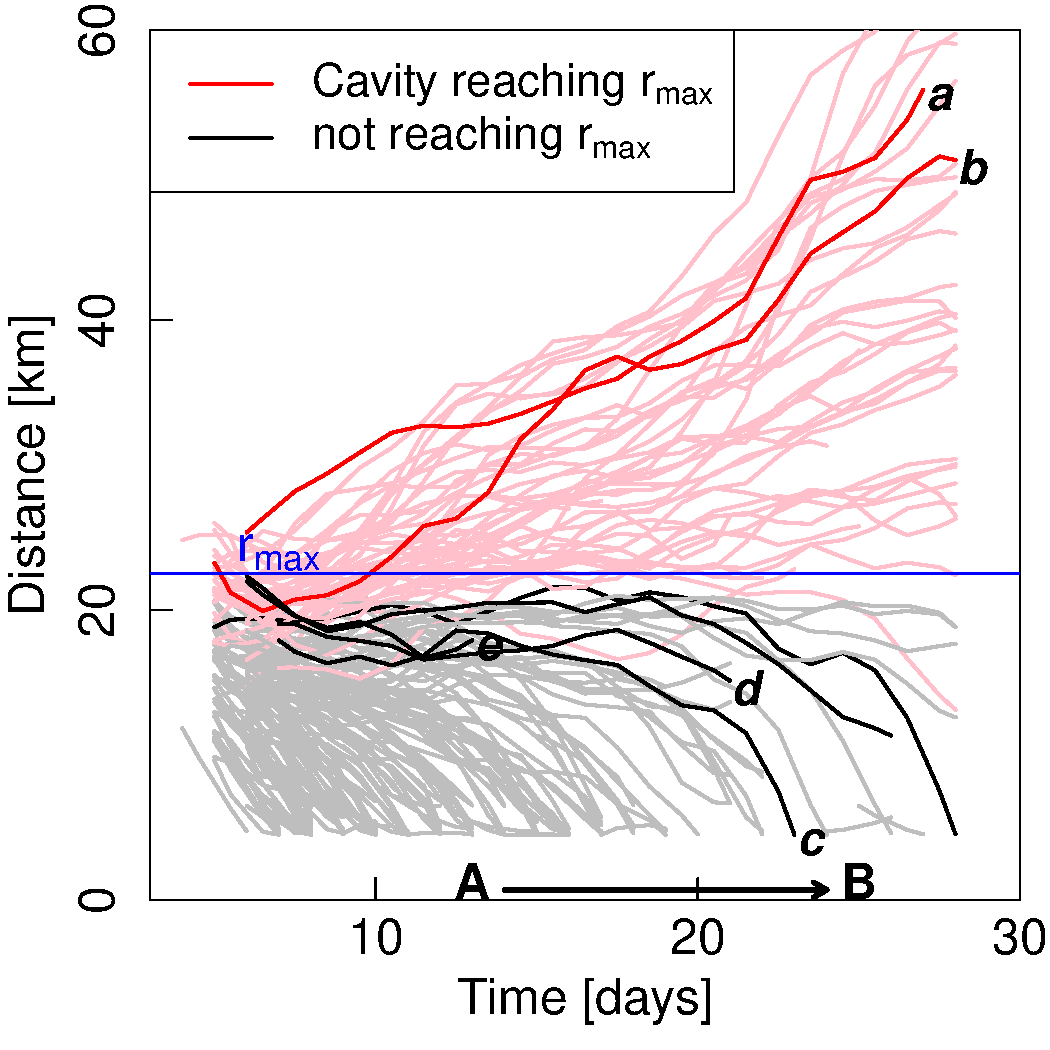
\includegraphics[height=0.32\linewidth]{size_evolution.pdf}
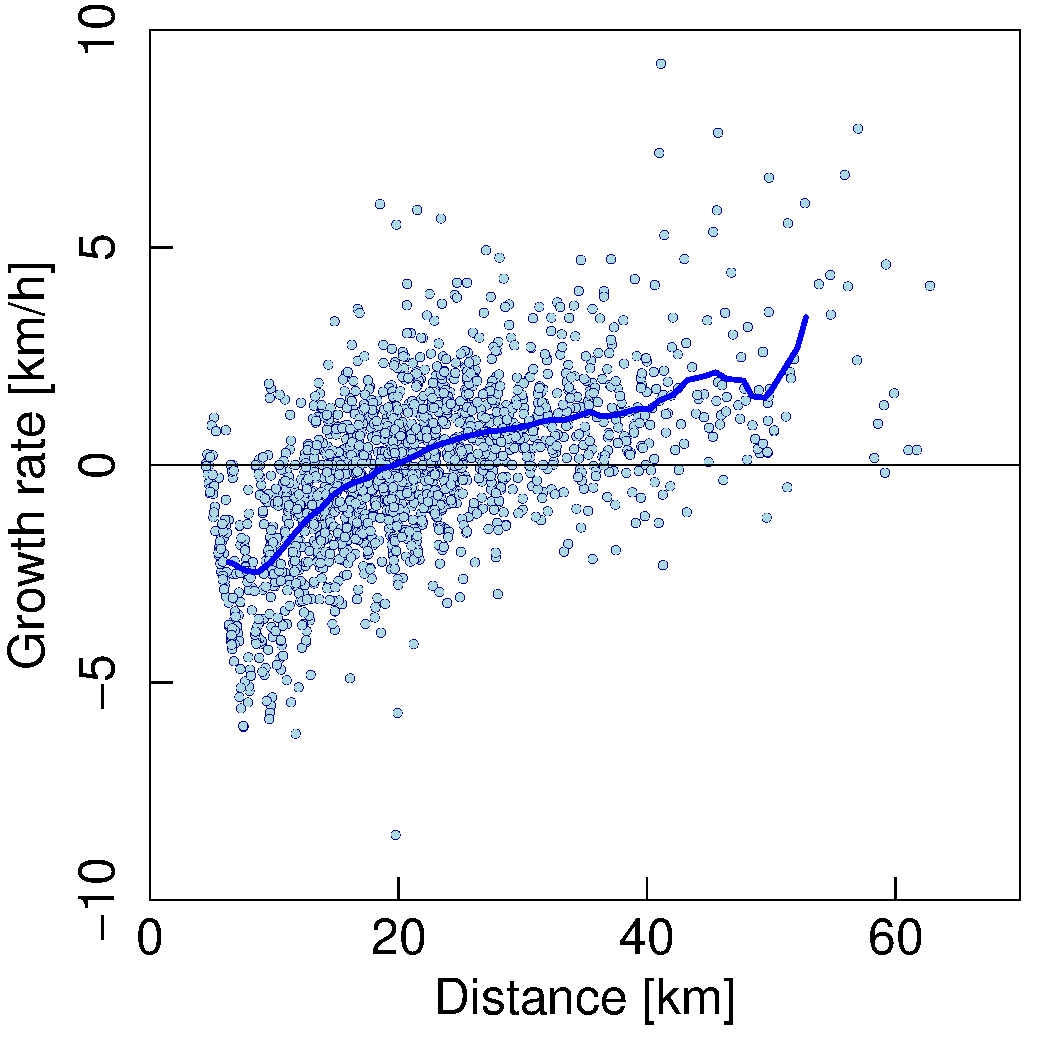
\includegraphics[height=0.32\linewidth]{growthrate_vs_size.pdf}}
%\end{overpic}
\caption{{\bf Cavities need a critical size to either grow or die}. (A--B) Five cavities ($a,b,c,d,e$) identified in LES data where black dots are the centers of the cold pools. (A) Cold pool centers at day 14. (B) Cold pool centers at day 24. Between these two time windows, cavities black letters ($b,c,d$) die out while red radii ($c,d$) grow further. (C) The size evolution of all cavities identified in this data set. Black cavities do not reach the critical size, $r_{\textnormal{max}}$, while red cavities do. {\color{red} Silas: Beautify the cold pool panel with the following suggestions: white background, grey wind field, clearly distinct bold and filled tracer colors, and remove color bar. Name the cavities incrementally after final cavity size: The three small $a,b,c$ and the two big $d,e$.}}
\label{fig:cavities}
\end{figure*}

\subsection{Transient line segments emerge in LES data}
When inspecting Fig.~\ref{fig:cavities}b,c, it is qualitatively apparent that some cells form line-like structures, a few of these are highlighted by arrows. 
To quantify, if such linear structures appear more frequently than would be expected at random, we introduce a measure, termed {\it line index}. 
In short, the line index is defined as the number of points involved in line segments. 
For a point to be involved in a line, it must not have more than two neighbors. 
A neighbor is another point, which is connected by the line of sight. ({\it Details:} Materials and Methods).
Fig.~\ref{fig:lines}.

\begin{figure*}
\centering
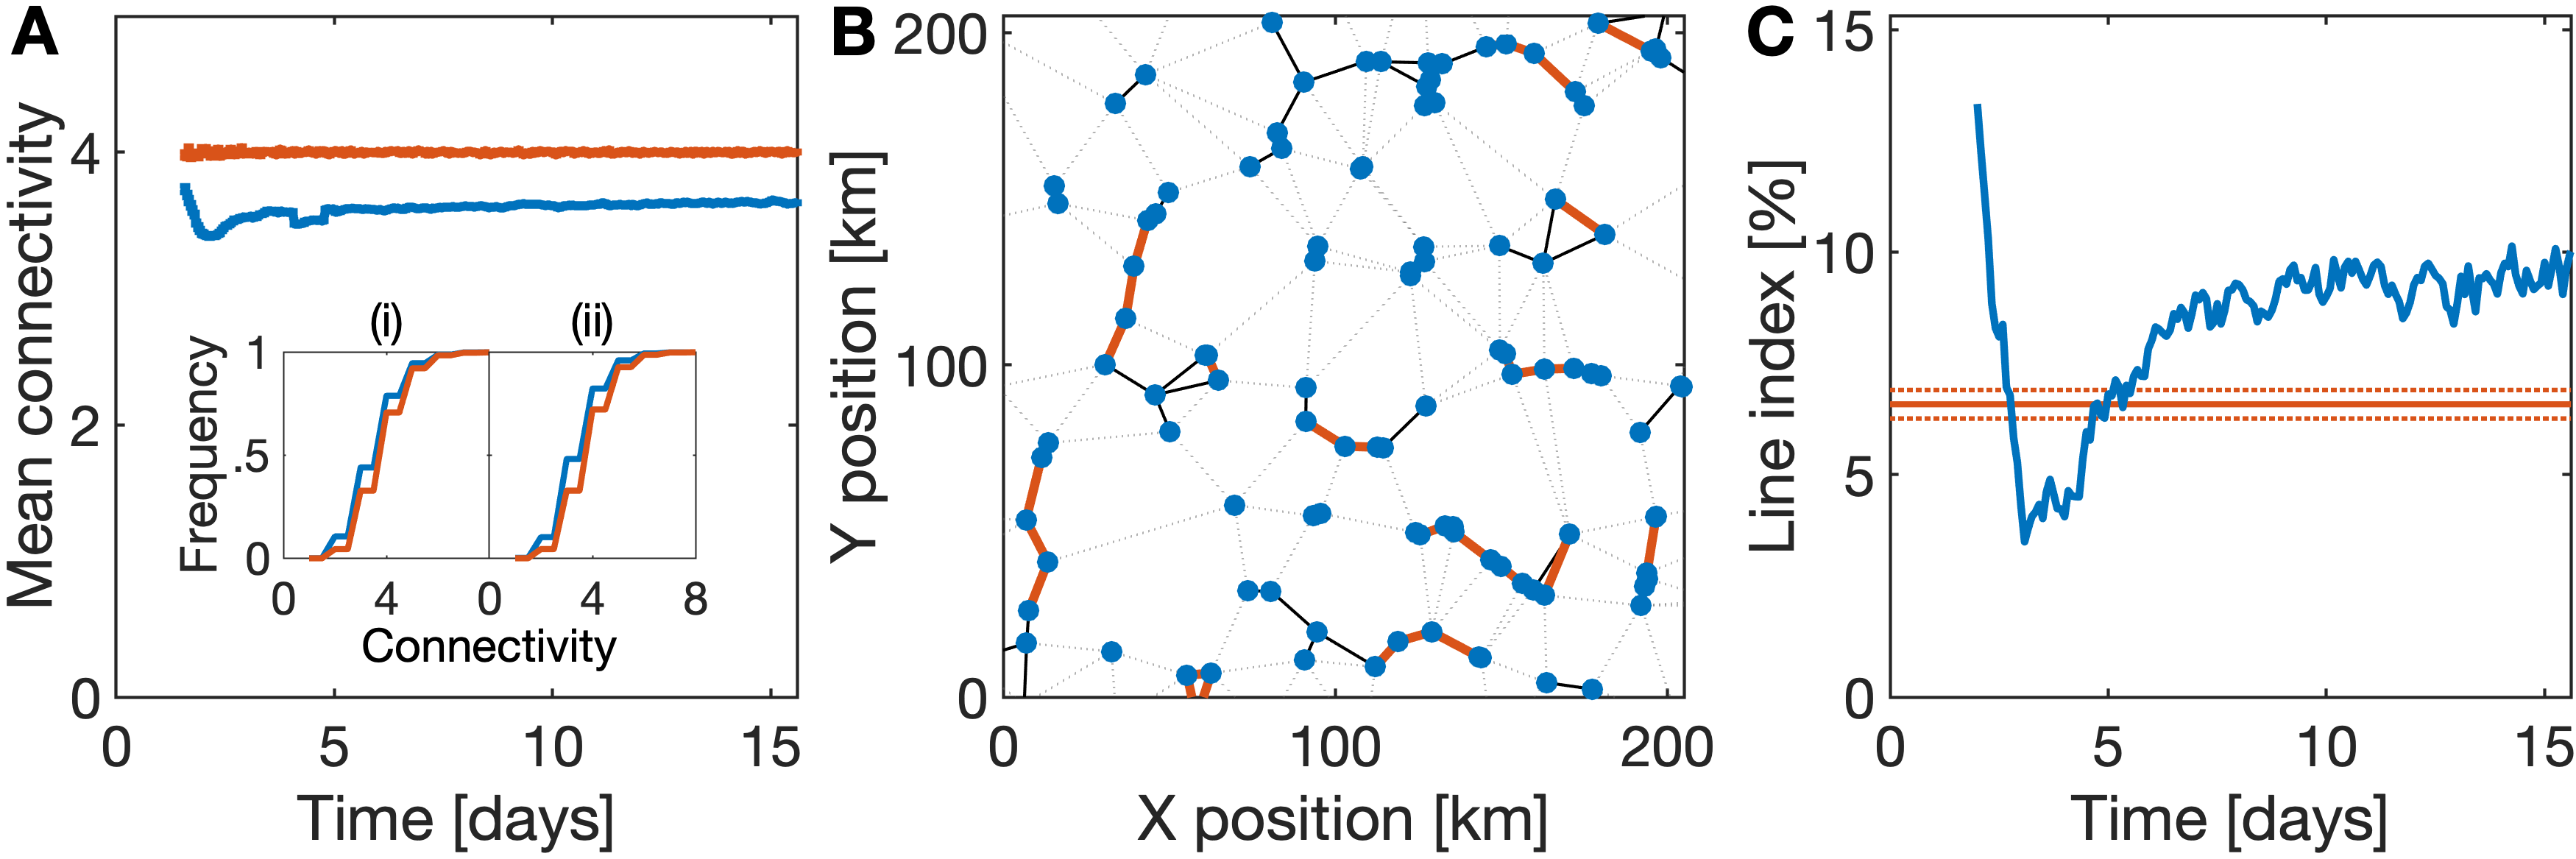
\includegraphics[height=0.3\linewidth]{linesNew}
\caption{{\bf Transient line segments emerge in LES data}. (A) Line segments (shown in red) identified by connecting cold pool centers (blue dots) at day 2. First, all line-of-sight connections are identified (dashed lines). Two points are within the line-of-sight if no other points are inside the smallest circle that includes the two points. Of these links only those that are shorter than the typical length $l=\sqrt{1/N}$ are preserved (black lines). Finally, only nodes with connectivity two counts as a line (red). A measure of the line index is achieved by dividing the number of nodes that obey these rules with the total number of nodes. (B) The line index as a function of time for the LES data (blue) and a randomized control data set with the same number of nodes (solid red line, dashed red lines illustrate the SEM). A sliding time window of 18 hours is applied. {\color{red} Silas: Add connectivity panel, and potentially add line index vs.~time window panel.}}
\label{fig:lines}
\end{figure*}

\subsection{Circle model captures line and cavity formation}
Some transition and realistic motivation...

In the case, the circles end up in the configuration shown in Fig.~\ref{fig:model}A, all subsequent generations induce three new circles that are located on a progressively smaller area. We avoid these singularities by introducing a minimum radius, $R_{\textnormal{min}}$, that circles need in order to replicate.

Fig.~\ref{fig:model}B, Fig.~\ref{fig:model}C, Fig.~\ref{fig:model}D.

\begin{figure*}
\centering
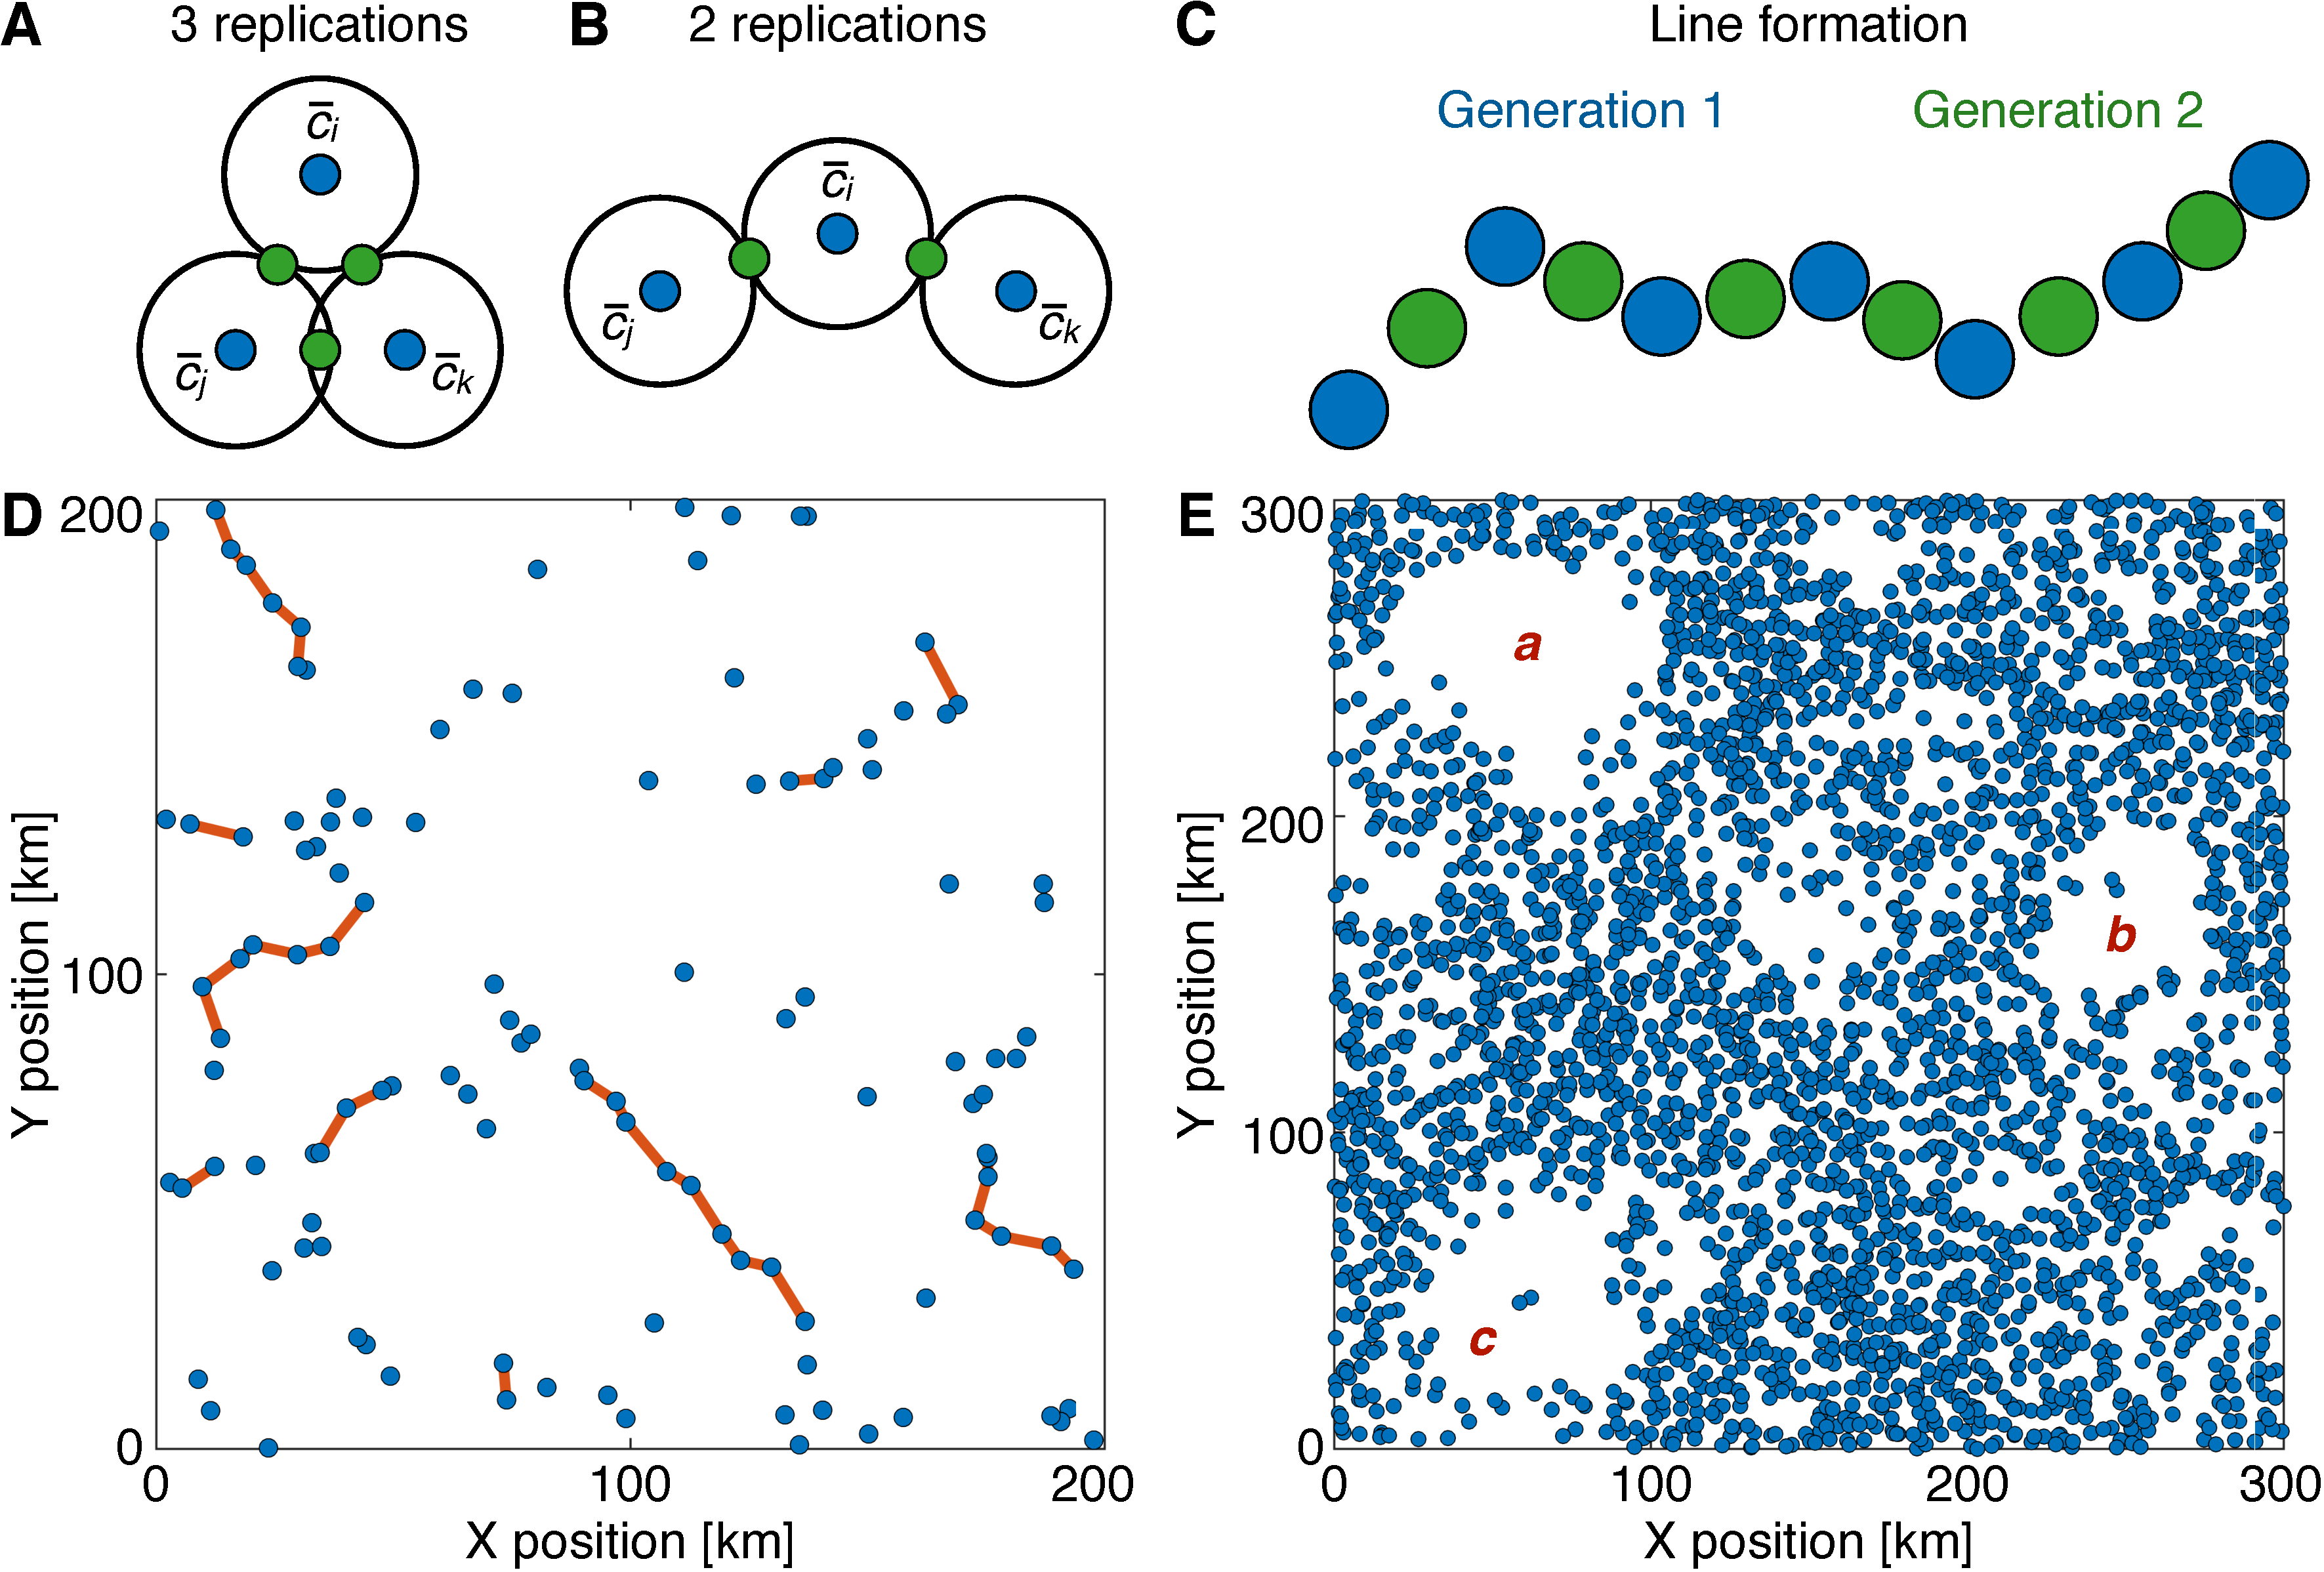
\includegraphics[height=0.5\linewidth]{model}
\caption{{\bf Circle model captures line and cavity formation}. (A--B) Three generation 1 circles (black) with centers at $\overline{c}_i, \overline{c}_j, \overline{c}_k$ (blue) grow with equal speed. Their collision points (green) initiate generation 2 circles. Either two or three circles are formed depending on the location of the original circles. (C) In the case multiple circles next to each other are in the configuration shown in (B), subsequent generations will form a progressively perfect line without noise. (D) Lines (red) connecting the circle centers (blue) are identified with the algorithm described in the caption to Fig.~\ref{fig:lines}A. (E) Three cavities ($a,b,c$) identified in a later time window of the simulation. Model parameters are $N=2000$, $R_{\textnormal{min}}=5$ km, $R_{\textnormal{max}}=30$ km, and $\eta=R_{\textnormal{min}}/2$. {\color{red} Silas: Add line index panel, and add cavity growth panel.}}
\label{fig:model}
\end{figure*}

\section{Discussion}
Discussion of the lines and cavities in the LES data. Squall lines.

Discussion of the main assumptions in the model: Constant and equal speed, circular shape, no CP1 or CP3 collisions, no time delay.

\section{Materials and Methods}
Here, we describe technical detail of the tracking of cavities, the tracking of cold pool gust fronts, the definition of the mathematical model, as well as the large eddy simulation setup.

\subsection{Tracking of cavities}\label{sec:cavity_tracking}
Cavities are tracked by first setting a time window $\Delta T_0$, over which the pattern of precipitation cell centers is to be observed.
A reasonable choice turns out to be $\Delta T_0=24$ $h$, as smaller values lead to too much noise along the edges of dry patches, while larger values do not properly warrant the dynamics of dry patches, i.e.~growth, decay and merging or splitting events.
Our conclusions do not depend on the precise value of $\Delta T_0$ (Fig.~\ref{fig:cavities_track_supp}).
%{\color{red} Silas: Would it be good to show this in supplement?}
For all precipitation cells falling into this time window, we identify the corresponding cell centers by the use of the iterative rain cell tracking method \cite{moseley2014}, yielding a collection of points $\mathbf{c}_i$ in space, where each point $\mathbf{c}_i \equiv (x_i, y_i)$ is a point in the two-dimensional plane.
We then scan the two-dimensional plane on the original LES grid of 2048 $\times$ 2048 points. 
For each point $\mathbf{c}$ on this grid we evaluate the distances $d_i(\mathbf{c})\equiv|\mathbf{c}-\mathbf{c}_i|$ to each cell center $\mathbf{c}_i$.
The distance $d(\mathbf{c})\equiv \min{\{d_i(\mathbf{c})\}}$ is then defined as the nearest distance of $\mathbf{c}$ to any of the centers $\mathbf{c}_i$. {\color{red} Silas: In reality, $d$ is the distance to the edge of a rain event, not to the center of a rain event.}

We now define the threshold distance $d_0\equiv 3.5$ $km$.
A cavity is defined as a contiguous region of points $\mathbf{c}$ with $d(\mathbf{c})>d_0$, that is, regions composed of points which are all located at distances larger than the threshold $d_0$ from existing precipitation cells.
$d_0$ is chosen as the approximate upper limit of distance fluctuations in the aggregated sub-region of the domain.
Doubling or halving this value would not have any implications for the conclusions drawn from the current study (Fig.~\ref{fig:cavities_track_supp}).
%{\color{red} Silas: Would it be good to show this in supplement?}

\subsection{Tracking of cold pools}\label{sec:cp_tracking}
Cold pool gust fronts are tracked similar to the particle method discussed in the recent literature \cite{haerter2018reconciling}:
in short, in any given time step particles are placed at the edges of existing precipitation cells. These particles are then advected along with the horizontal velocity field.

\subsection{Mathematical model}\label{sec:math_model}
$N$ points are initialized on a 2D domain of 1000 x 1000 km size with double periodic boundary conditions. These points are called generation 1. All points grow with equal and constant speed. The growing circles have centers at $\overline{c}_i=[x_i, y_i]$ and radii $r_i$. The collision point, [$x, y$], between two circles is determined by solving
\begin{equation}
    (x-x_i)^2 + (y-y_i)^2 = (r_i+dr)^2,
\end{equation}

and 
\begin{equation}
    (x-x_j)^2 + (y-y_j)^2 = (r_j+dr)^2,
\end{equation}

where $dr$ is the distance from the circles' rim to the collision point. Only collisions that fall on the straight line between the two circle centers are allowed (Fig.~\ref{fig:model}A--B). This is defined by the linear constraint that {\color{red} Silas: we need an atmospheric argument for this}
\begin{equation}
    y = \frac{x - x_i}{x_j - x_i} (y_j - y_i) + y_i.
\end{equation}

This gives three equations (Eq.~1--3) with three unknowns ($x, y, dr$). Generally, this set of equations has two solutions. However, we do not allow cold pools to shrink, and therefore only positive real solutions are valid.

For each generation a list of all potential collision points are calculated, and this list is sorted incrementally by $dr$. The system is updated by inserting generation 2 circles at the collision points in the order they appear. Circles are only inserted if that location is not already taken by the subsequent generation. This process is repeated until no more collisions occur.

To make the model more realistic, we introduce a minimum radius, $R_{\textnormal{min}}$, and a maximum radius, $R_{\textnormal{max}}$, that circles need in order to replicate. Furthermore, we introduce noise on the collision point taken from a normal distribution with the width $\eta$. {\color{red} Silas: Mention where you shift the system by an infinitesimal small value $\epsilon=2^{-52}$.}

\section*{Acknowledgments}\label{sec:acknowledgments}
We thank S.~J.~Boeing for useful comments, and Cathy Hohenegger for providing her RCE simulation results.
SBN acknowledges funding through the Danish National Research Foundation (grant number: DNRF116).
JOH gratefully acknowledges funding by a grant from the VILLUM Foundation (grant number: 13168) and the European Research Council (ERC) under the European Union's Horizon 2020 research and innovation program (grant number: 771859).

\bibliography{references_SB.bib}

\setcounter{figure}{0} 
\renewcommand{\thefigure}{S\arabic{figure}}

\begin{figure*}
\centering
%\begin{overpic}
%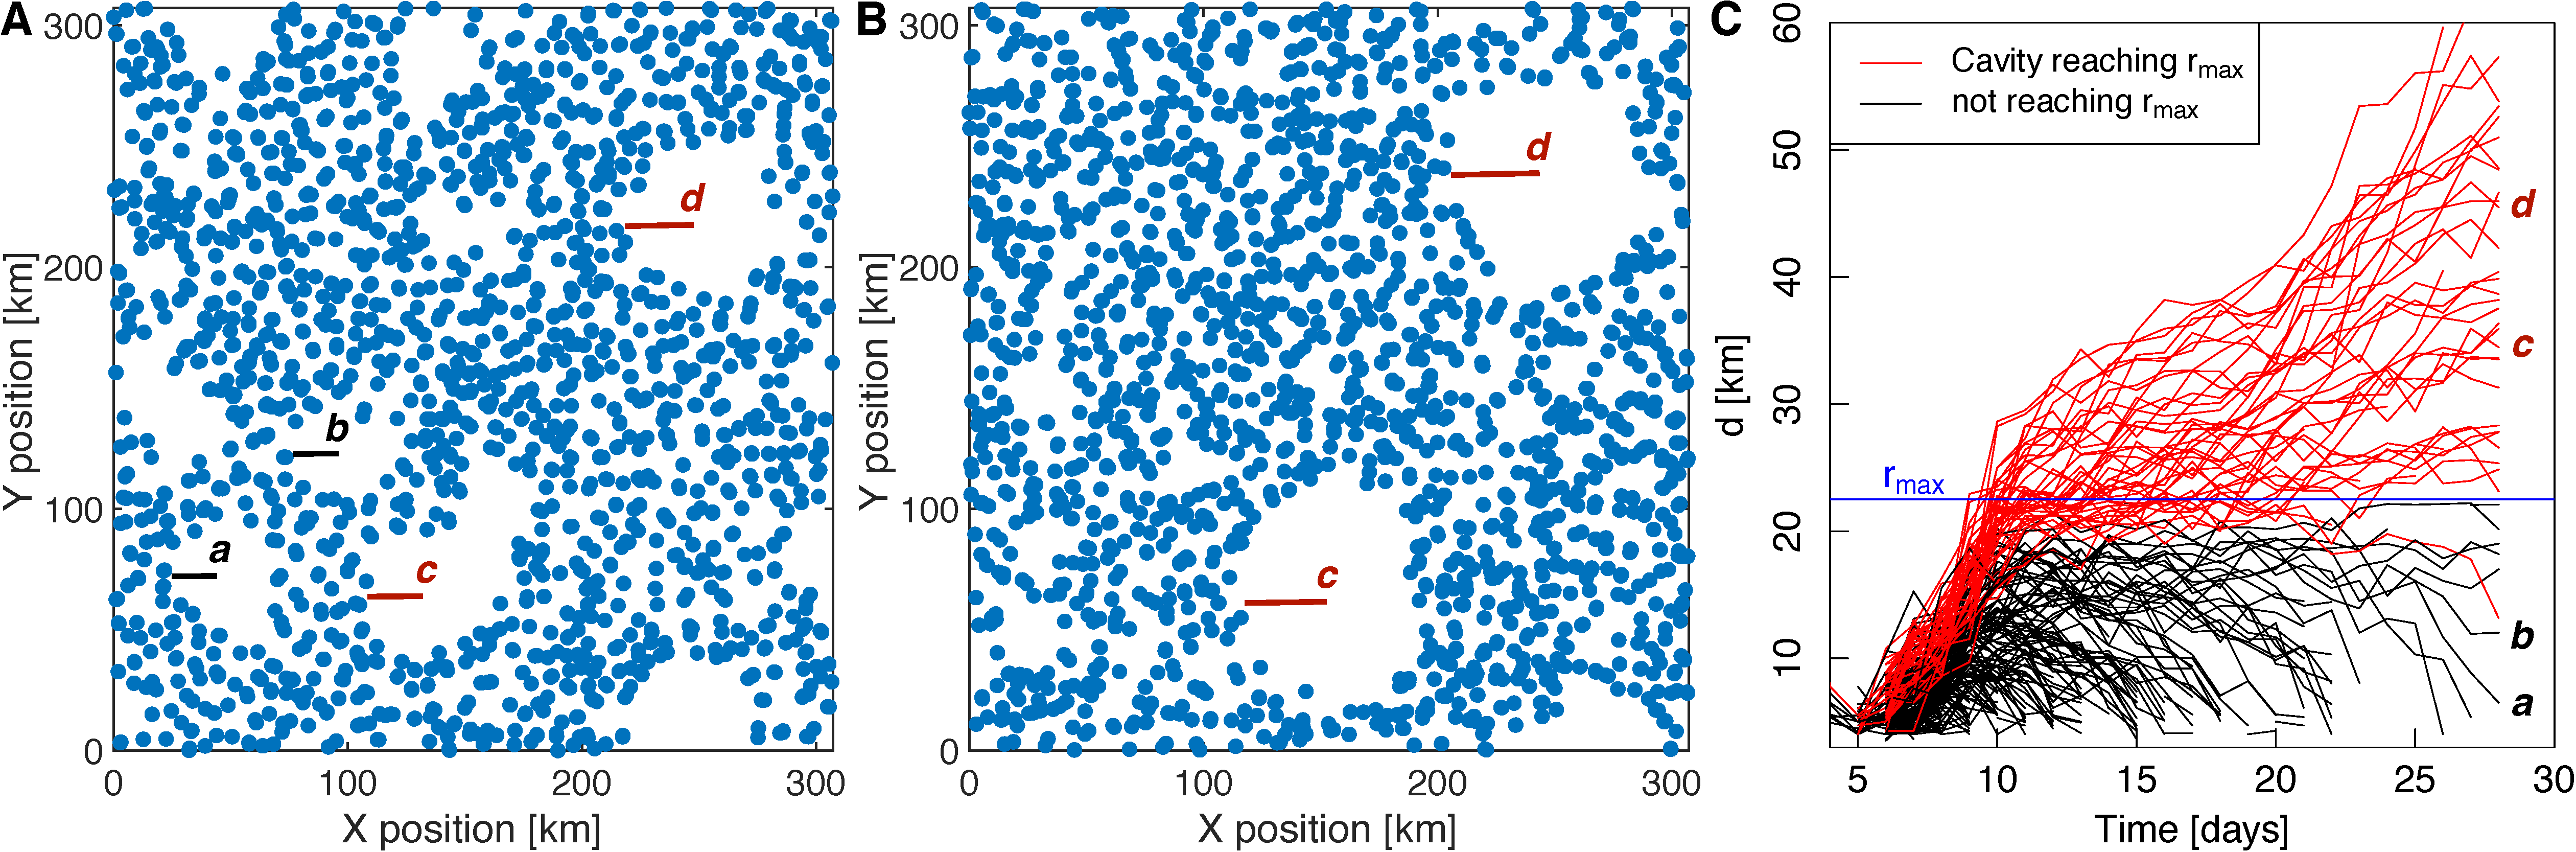
\includegraphics[height=0.33\linewidth]{cavities}
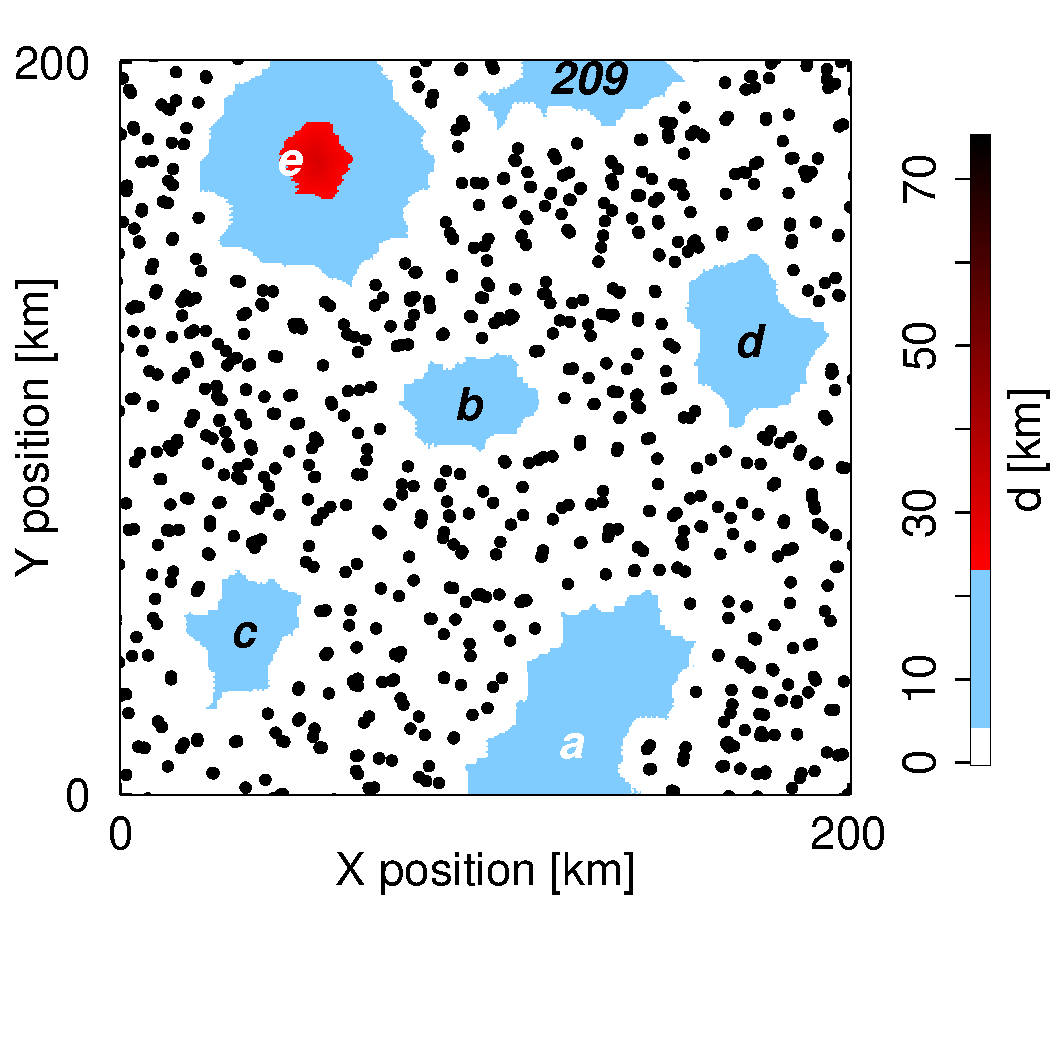
\includegraphics[trim={0 0 1.8cm 0},clip,height=0.32\linewidth]{distance_12.pdf}
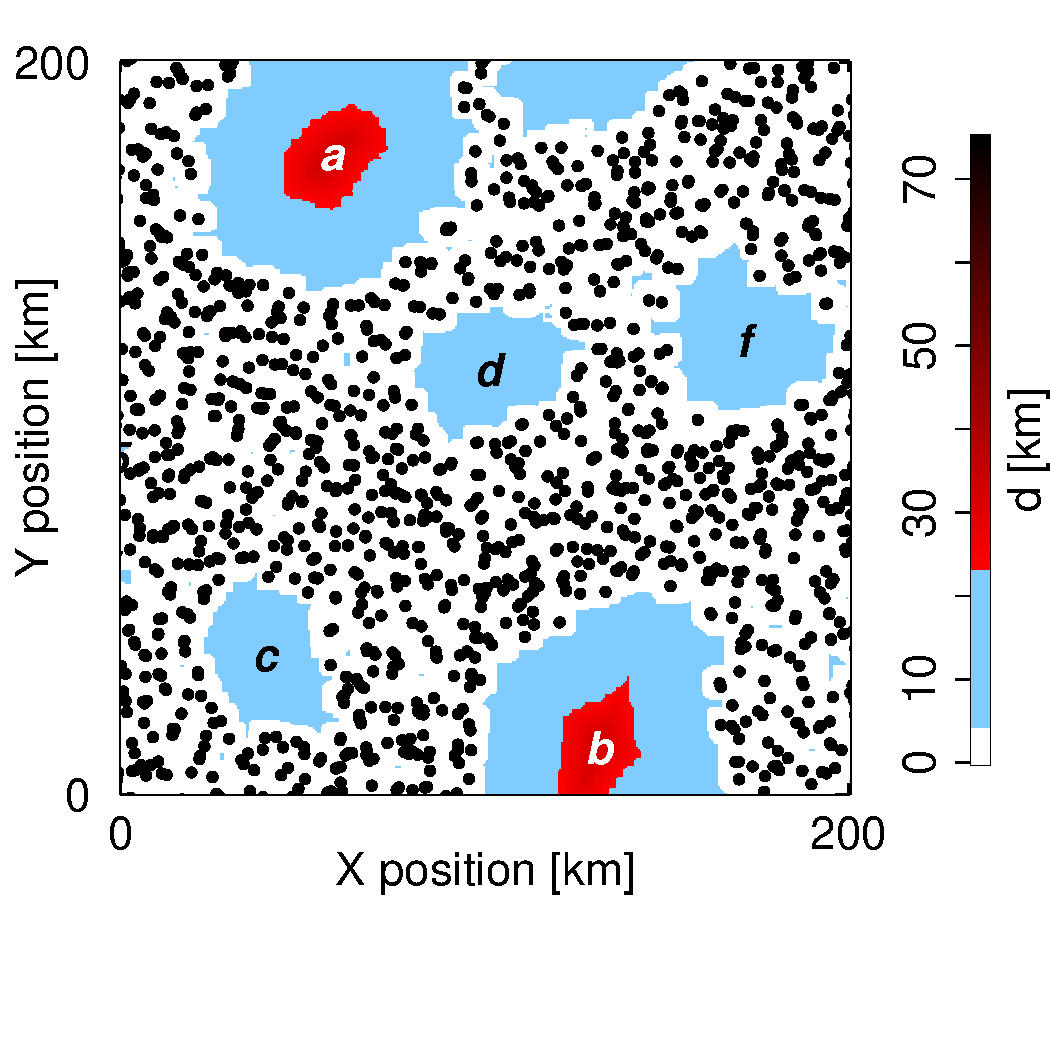
\includegraphics[trim={0cm 0 1.8cm 0},clip,height=0.32\linewidth]{distance_15.pdf}
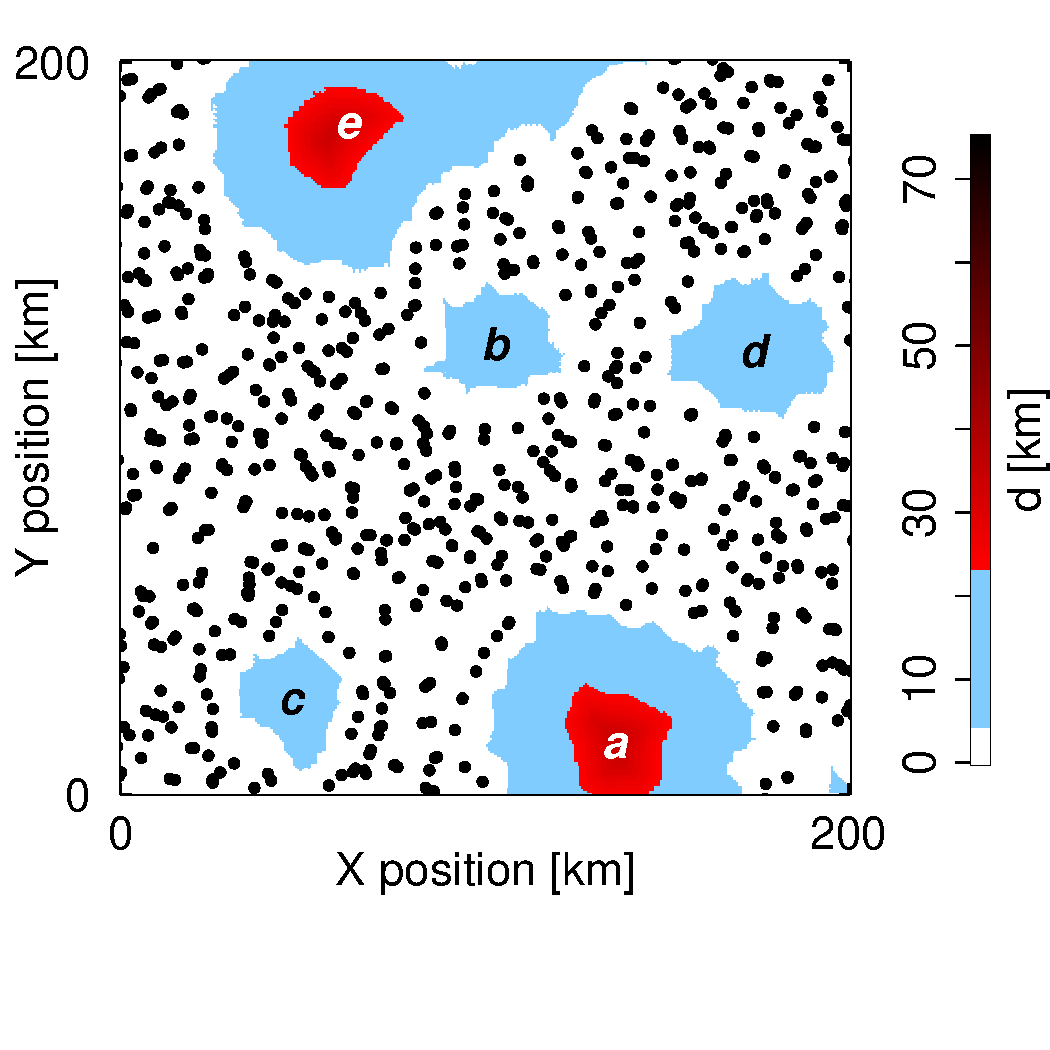
\includegraphics[trim={0 0 1.8cm 0},clip,height=0.32\linewidth]{distance_18.pdf}
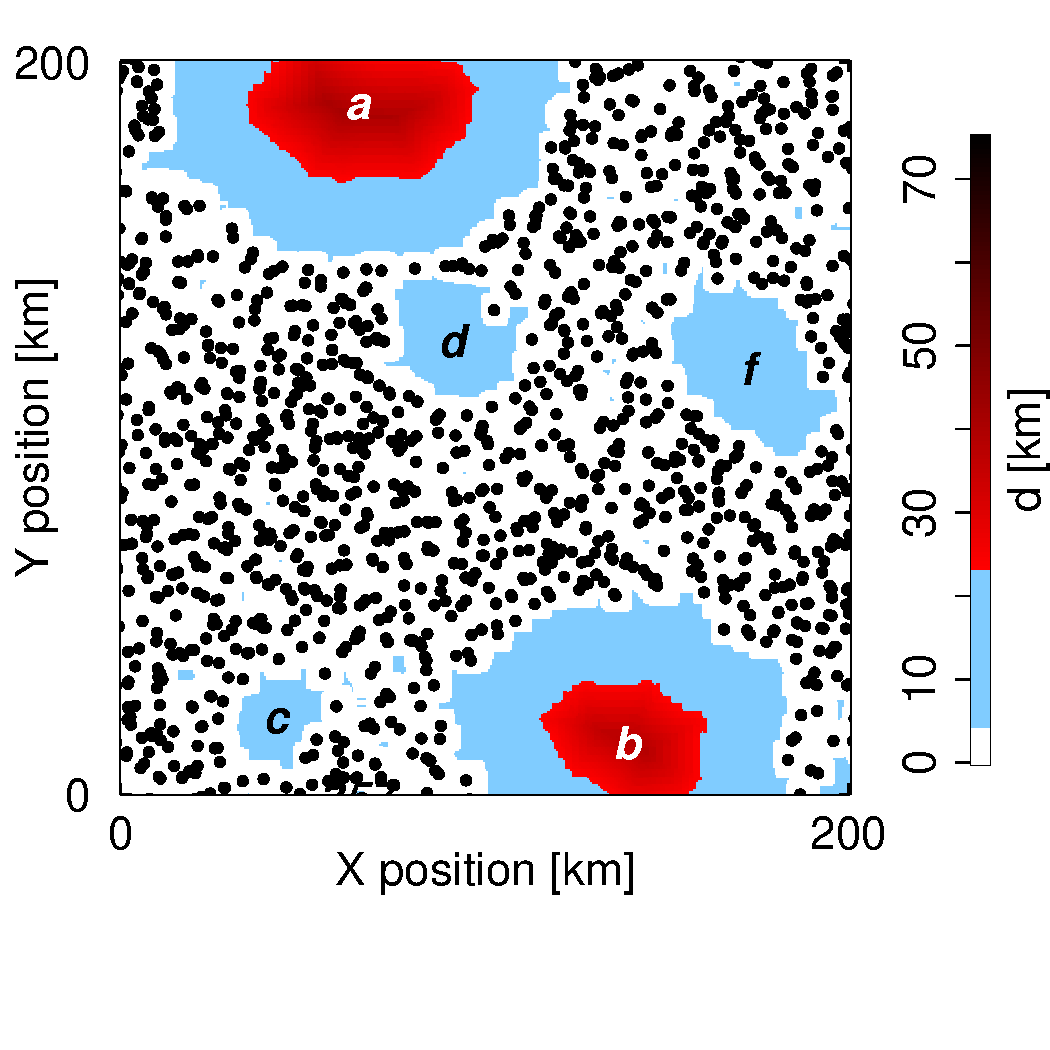
\includegraphics[trim={0 0 1.8cm 0},clip,height=0.32\linewidth]{distance_21.pdf}
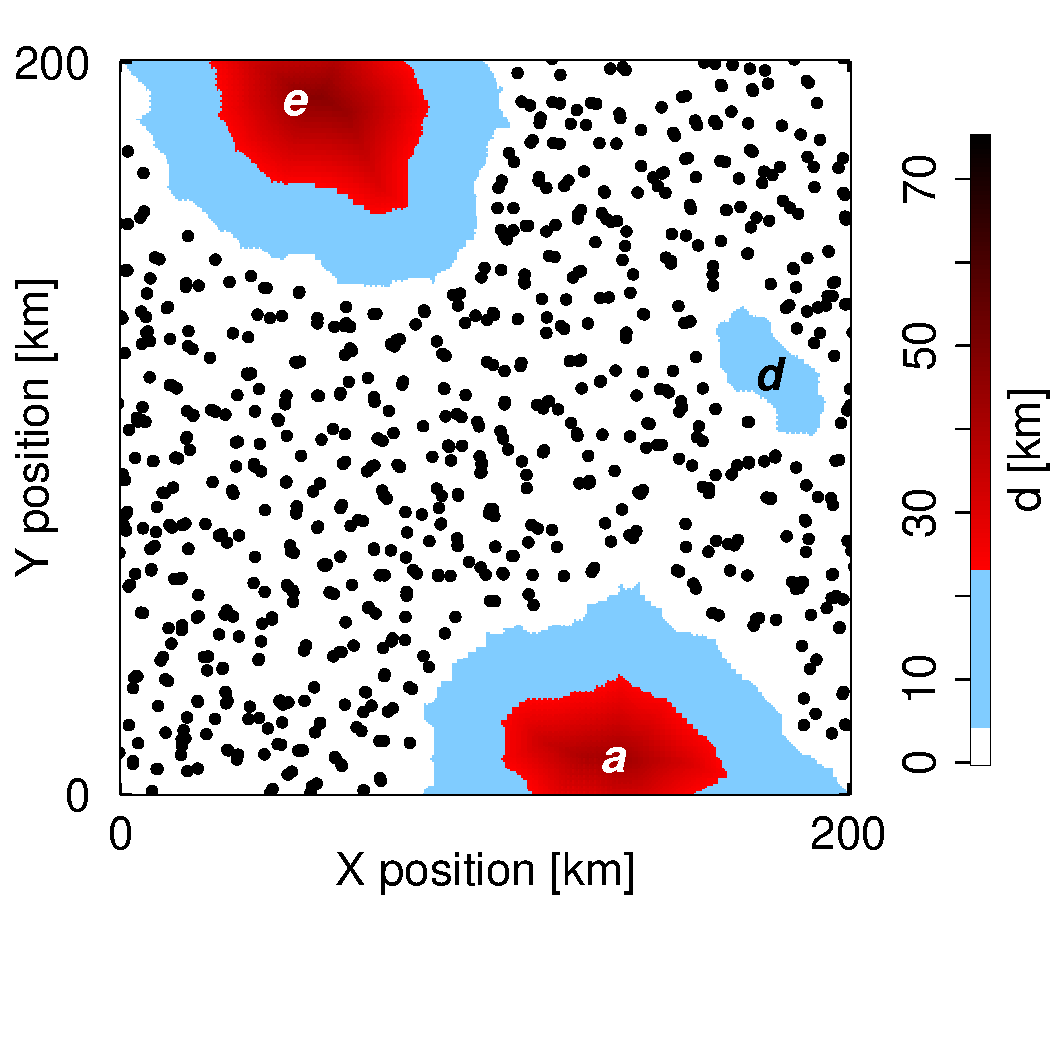
\includegraphics[trim={0 0 1.8cm 0},clip,height=0.32\linewidth]{distance_24.pdf}
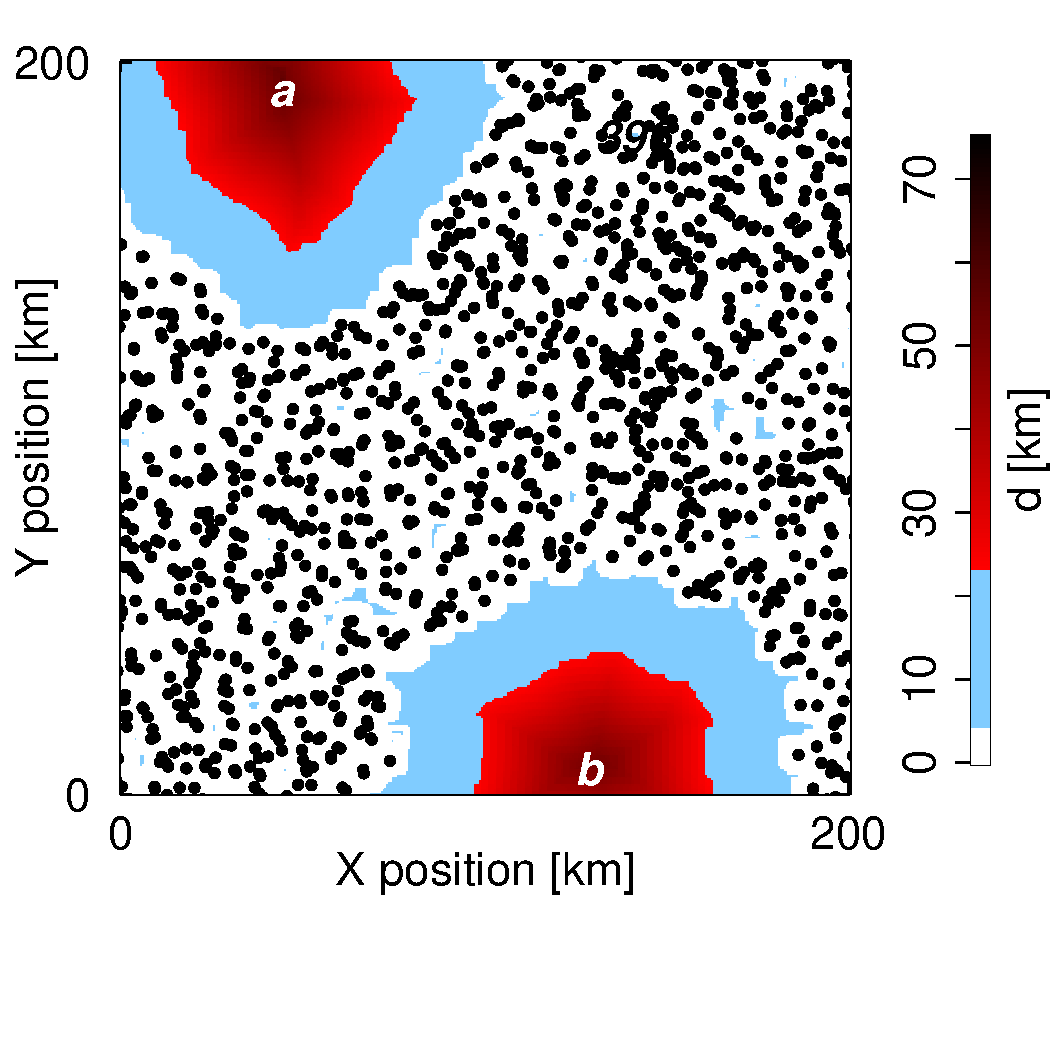
\includegraphics[trim={0 0 1.8cm 0},clip,height=0.32\linewidth]{distance_27.pdf}
%\end{overpic}
\caption{{\bf Patterns of cells at various times during self-aggregation.}}
\label{fig:cavities_supp}
\end{figure*}


\begin{figure*}
\centering
%\begin{overpic}
%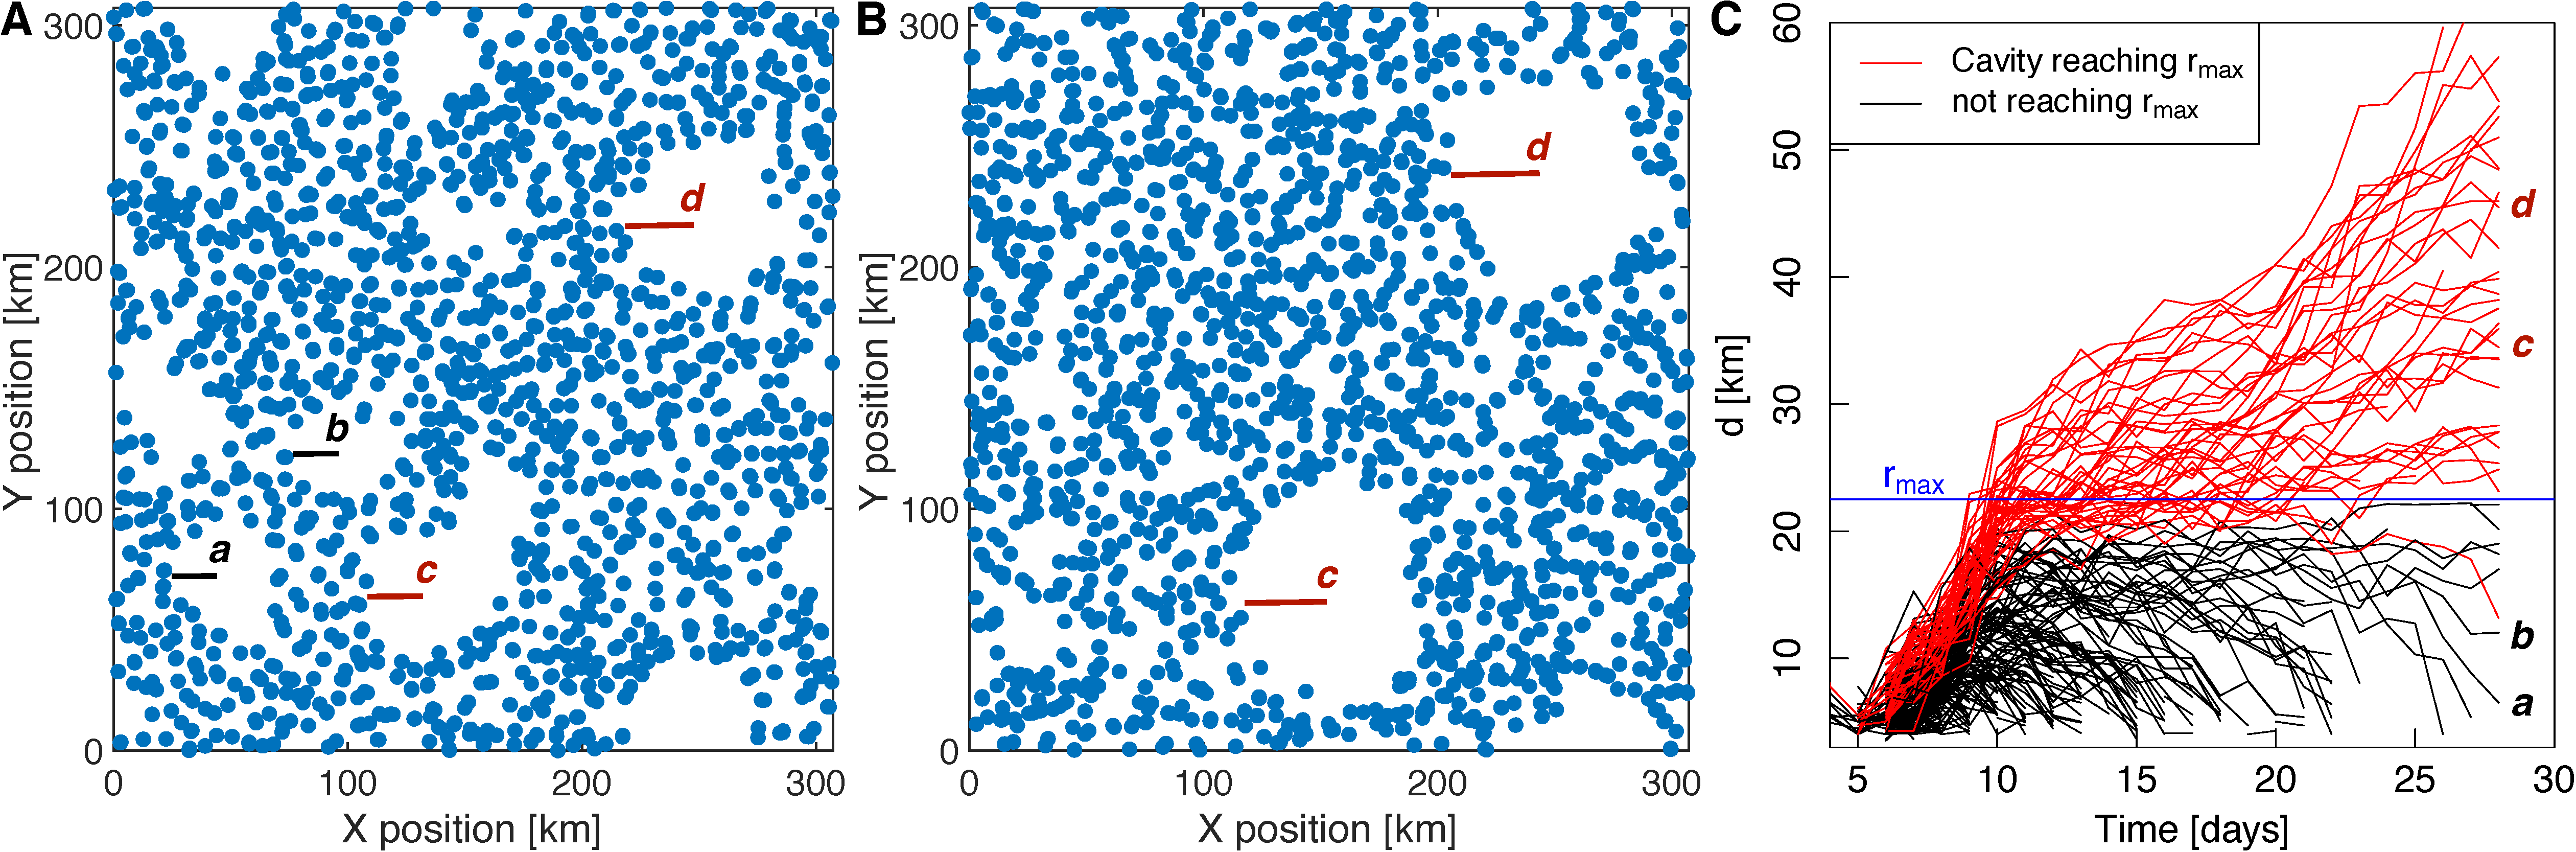
\includegraphics[height=0.33\linewidth]{cavities}
%\end{overpic}
\caption{{\bf Tracked cavities for a different choice of time window $\Delta T_0$.}}
\label{fig:cavities_track_supp}
\end{figure*}

\end{document}